\subsection{Documentación e Implementación de los bloques VCO}
Tras inspeccionar el código fuente de los bloques incrustados en GNU Radio, se redefinió la documentación interna para reflejar fielmente el comportamiento matemático descrito en la metodología.

\begin{figure}[H]
    \centering
    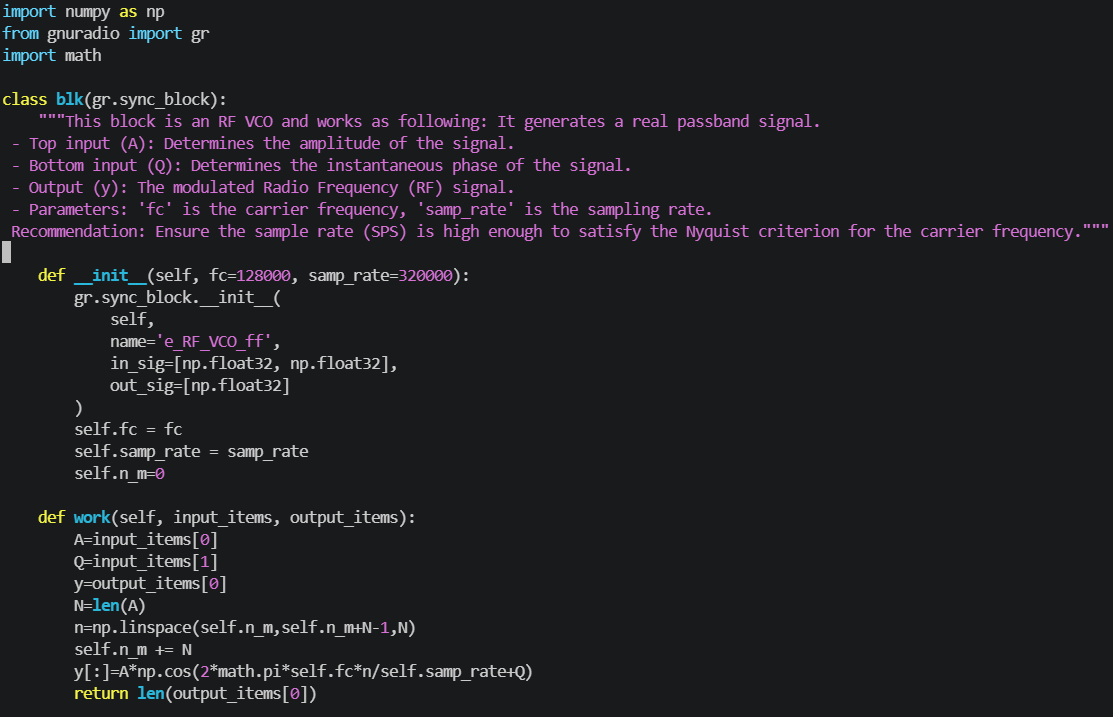
\includegraphics[width=0.48\textwidth]{imagenes/vco_rf.png}
    \caption{Código interno modificado para el bloque de Radiofrecuencia (e\_RF\_VCO\_ff).}
    \label{fig:codigo_vco_rf}
\end{figure}

Como se observa en la Figura \ref{fig:codigo_vco_rf}, la ayuda documentada en inglés estipula explícitamente: \textit{"This block is an RF VCO and works as following: It generates a real passband signal. Top input (A): Determines the amplitude of the signal. Bottom input (Q): Determines the instantaneous phase of the signal. Output (y): The modulated Radio Frequency (RF) signal. Recommendation: Ensure the sample rate (SPS) is high enough to satisfy the Nyquist criterion for the carrier frequency."}

De manera análoga, se configuró el bloque para la Envolvente Compleja (Figura \ref{fig:codigo_vco_ec}):

\begin{figure}[H]
    \centering
    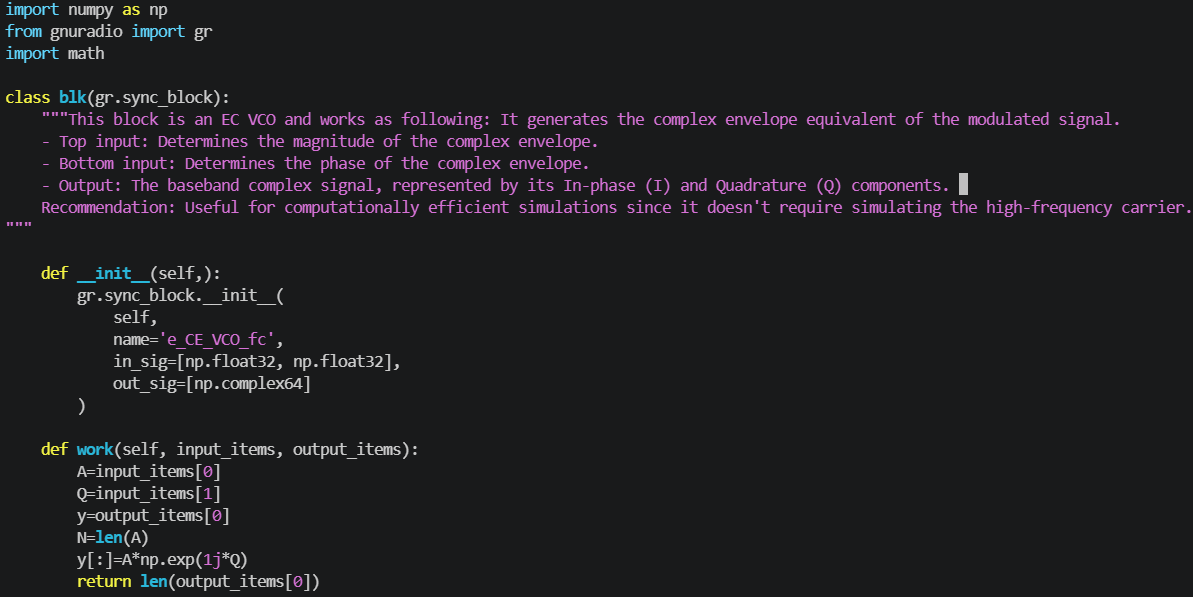
\includegraphics[width=0.48\textwidth]{imagenes/vco_ec.png}
    \caption{Código interno modificado para el bloque de Envolvente Compleja (e\_EC\_VCO\_fc).}
    \label{fig:codigo_vco_ec}
\end{figure}

La documentación implementada para la EC indica: \textit{"This block is an EC VCO and works as following: It generates the complex envelope equivalent of the modulated signal. Top input: Determines the magnitude of the complex envelope. Bottom input: Determines the phase of the complex envelope. Output: The baseband complex signal. Recommendation: Useful for computationally efficient simulations since it doesn't require simulating the high-frequency carrier."}